\section{\ref{rq:type-visualisation} How to visualise change?} \label{rq:type-visualisation-answer}
In section \ref{sec:finding-changes} the detection of changes between two version of the same application is explained. It showed that having two models the abstract states were compared to find corresponding states. The corresponding states were compared to discover the changes in element data. In this setion the change detection results is used as input for visualising the changes. 

In this section the visualisation of the change detection results are discussed. First the technology is discussed how to show a graph and what is needed for that (section \ref{sec:graph-visualisation}). In section \ref{sec:merge-graph} is explained how the results are used to merge the two graphs and to visualise one single graph.

\subsection{How are graphs visualised} \label{sec:graph-visualisation}

All the information about a model and graph is stored in OrientDB. The new Analysis website is retrieving the model and graph data through the \testar .NET server from the OrientDB database. This communication is done by the \verb|GraphEngine|. The \verb|GraphEngine| contains a method for each layer it, for example: \verb|FetchAbstractLayerAsync|. Edges between layers are retrieved with a different method, for example: \verb|FetchAbstractConcreteConnectors| which retrieves the edges between a abstract and concrete state. By splitting up the method for each layer it becomes possible to only retrieve the information that is needed. As an example, the graph shown for an application, like in figure \ref{fig:graph-page}, needs to have all the information while the detection algorithm only needs the abstract information. 

The \verb|GraphEngine| is returning the information as a list of \verb|GraphElement|'s. Each graph element contains all the data about either a node, an edge or a compound object. A compound object is served as a parent in which other element can be visualised. An example of a compound layer can be found in figure .... \todo{Add picture with a compound layer} and is used to group nodes together.  

The list is serialised into a JSON format structure. An example of the serialisation result can be viewed in listing \ref{code:graph-json}. The data contains an array of elements each having three attributes: \verb|group|, \verb|data| and \verb|classes|. The group is either contains the value nodes or edges, representing their graph element. The attribute \verb|data| contains the \verb|id| of the element and all the additional data about the vertex/edge. For an edge that data also contains the target and source id, specifying the id of a vertex. The element classes is similar as classes in \textsc{CSS} and can be used to style the elements in the GUI. 

The result of listing \ref{code:graph-json} generates the graph visible in figure \ref{fig:graph-example} \todo{Add footnote with live example and reference the appendix for the code.}

\begingroup
\captionsetup{type=figure}
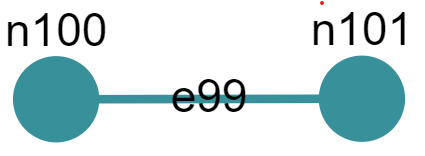
\includegraphics[scale=0.6]{content/5-Results/Images/graph-example.png}
\captionof{figure}{Example graph}\label{fig:graph-example}
\endgroup

data is loading from the server. \verb|GraphEngine| is used. Contains methods for each 
all the elements are in a moved into a model format. The model is already shown in figure \ref{fig:class-diagram-models}. The class \verb|AppGraph| does not play a role in the displaying the graph. 

The \verb|List| with \verb|GraphElement| are transformed into a JSON format. Listing \ref{code:graph-json} gives an example a graph in json format. 

There are two groups, nodes and edgeds. 

Crytoscape is used for the visualisation of the graph 
explain graph input.. state and connectors 

An graph is a combination of nodes and edges, this can be represented in

e stands for edge
n stands for node

\newpage
\begin{lstlisting}[language=xml, caption=Graph representation in JSON, label=code:graph-json]
[
  {
    "group": "nodes",
    "data": {
      "id": "n100" 
    },
    "classes":[
      "AbstractState"
    ]
  },
  {
    "group": "nodes",
    "data": {
      "id": "n101"
    },
    "classes":[
      "AbstractState"
    ]
  },
  {
    "group": "edges",
    "data": {
      "id":"e99",
      "target": "n100",
      "source": "n101"
    },
    "classes" :[
      "AbstractAction"
    ]
  }
]
\end{lstlisting}

\subsection{Merging the two graphs} \label{sec:merge-graph}

put place of the GraphEngine here

within with items from $G_{old}$ then iterate though $G_{new}$ items


explain the graph input basics

clean up of data from the change detection


classes indicated how to show it in the UI
Id = is the id of the node or edge
source and target is used for edge to connect to a node in the UI
rest of the data is data from \testar

corresponding state only need to come from $G_{new}$ since those states contains the change detection result information. We though need to import all the other states from $G_{old}$ since thouse are the removed states. We find the removed states by looking which state does are missing the \verb|CD_CorrespondingId| element data. 


Andrews et al. show in \cite{andrews2009visual} how to graphs can be merged. They lay out six steps to two graphs are merged into a merge graph. 


from the $G_n$ and $G_o$ the merge graph $G_m$ is created. 
%% do not indent code since it indents its extra in the LaTeX output

to create a matching list, the corresponding states are first loading into a matrix 